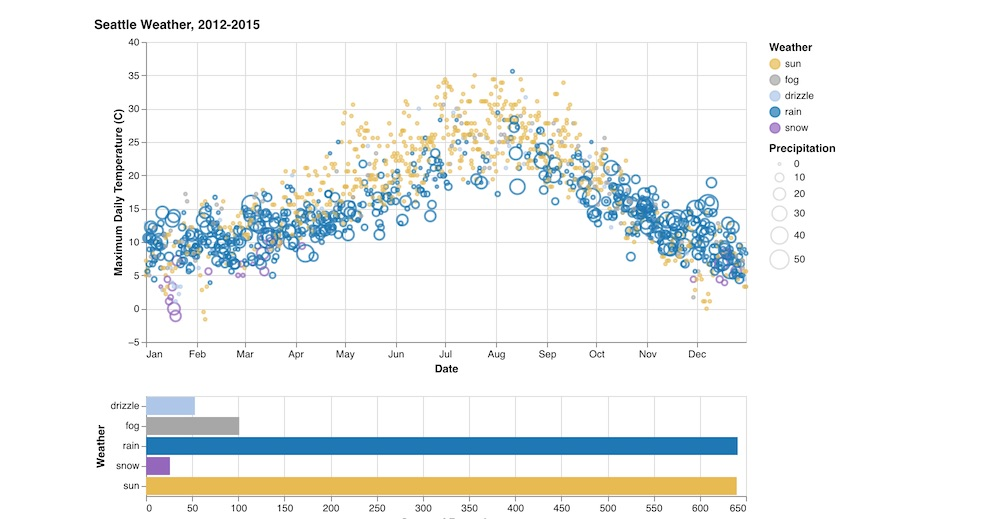
\includegraphics{assets/vega-chart.jpg} \emph{Scatterplot and horizontal
box plot}

\href{https://vega.github.io/vega-lite/}{Vega-Lite} is an interactive
charting library that uses a well-regarded declarative syntax for
defining charts known as ``Grammar of Graphics''.

See the Vega-Lite website for many examples of typical data
visualizations that are possible: the usual bar-charts, scatterplots,
and much more are possible.

\textbf{NOTE:} For simple bar, area, and line charts, you will probably
be better off using the simple charts defined in
\href{bar-area-line}{Bar, Area, and Line Charts}

\hypertarget{dashboards}{%
\subsection{Dashboards}\label{dashboards}}

Vega-lite charts can be embedded in dashboards using
\texttt{type:\ vega} and specifying the config details in the props as
follows:

\begin{Shaded}
\begin{Highlighting}[]
\FunctionTok{row}\KeywordTok{:}
\AttributeTok{  }\KeywordTok{{-}}\AttributeTok{ }\FunctionTok{title}\KeywordTok{:}\AttributeTok{ My Vega Chart}
\AttributeTok{    }\FunctionTok{type}\KeywordTok{:}\AttributeTok{ vega}
\AttributeTok{    }\FunctionTok{config}\KeywordTok{:}\AttributeTok{ my{-}example.vega.json}
\end{Highlighting}
\end{Shaded}

\hypertarget{usage}{%
\subsection{Usage}\label{usage}}

A file named \texttt{*.vega.json} must be present in working folder.
Each json file matching that pattern will produce a separate Vega-Lite
diagram.

\textbf{DATA} can either be an array of hard-coded values (see
\texttt{example.vega.json}) or a URL pointing to a file containing an
array of JSON or CSV data as in \texttt{movies.vega.json}. The file
format is guessed based on the file extension.

See \href{https://vega.github.io/vega-lite/docs/data.html}{Data in Vega}
for the full story on what data types are supported by Vega.

\begin{itemize}
\tightlist
\item
  If the URL is pointing to a file in the local filestorage, the plugin
  will load it directly and embed the data in the object automatically.
\item
  If the URL is a fully-qualified URL, the Vega library will load it on
  its own.
\end{itemize}

\textbf{AUTOSIZE} must be set as in the example below for the charts to
be responsive to window size changes.

\textbf{WIDTH} and \textbf{HEIGHT} can be hardcoded to pixel sizes, but
a width set to \texttt{container} will be responsive. Height needs to be
specified.

\begin{center}\rule{0.5\linewidth}{0.5pt}\end{center}

\textbf{example.vega.json}

\begin{Shaded}
\begin{Highlighting}[]
\FunctionTok{\{}
  \DataTypeTok{"$schema"}\FunctionTok{:} \StringTok{"https://vega.github.io/schema/vega{-}lite/v4.json"}\FunctionTok{,}
  \DataTypeTok{"data"}\FunctionTok{:} \FunctionTok{\{} \DataTypeTok{"url"}\FunctionTok{:} \StringTok{"movies.json"} \FunctionTok{\},}
  \DataTypeTok{"transform"}\FunctionTok{:} \OtherTok{[}
    \FunctionTok{\{}
      \DataTypeTok{"filter"}\FunctionTok{:} \FunctionTok{\{}
        \DataTypeTok{"and"}\FunctionTok{:} \OtherTok{[}
          \FunctionTok{\{} \DataTypeTok{"field"}\FunctionTok{:} \StringTok{"IMDB Rating"}\FunctionTok{,} \DataTypeTok{"valid"}\FunctionTok{:} \KeywordTok{true} \FunctionTok{\}}\OtherTok{,}
          \FunctionTok{\{} \DataTypeTok{"field"}\FunctionTok{:} \StringTok{"Rotten Tomatoes Rating"}\FunctionTok{,} \DataTypeTok{"valid"}\FunctionTok{:} \KeywordTok{true} \FunctionTok{\}}
        \OtherTok{]}
      \FunctionTok{\}}
    \FunctionTok{\}}
  \OtherTok{]}\FunctionTok{,}
  \DataTypeTok{"mark"}\FunctionTok{:} \StringTok{"rect"}\FunctionTok{,}
  \DataTypeTok{"width"}\FunctionTok{:} \StringTok{"container"}\FunctionTok{,}
  \DataTypeTok{"height"}\FunctionTok{:} \DecValTok{300}\FunctionTok{,}
  \DataTypeTok{"autosize"}\FunctionTok{:} \FunctionTok{\{} \DataTypeTok{"type"}\FunctionTok{:} \StringTok{"fit"}\FunctionTok{,} \DataTypeTok{"resize"}\FunctionTok{:} \KeywordTok{true} \FunctionTok{\},}
  \DataTypeTok{"encoding"}\FunctionTok{:} \FunctionTok{\{}
    \DataTypeTok{"x"}\FunctionTok{:} \FunctionTok{\{}
      \DataTypeTok{"bin"}\FunctionTok{:} \FunctionTok{\{} \DataTypeTok{"maxbins"}\FunctionTok{:} \DecValTok{60} \FunctionTok{\},}
      \DataTypeTok{"field"}\FunctionTok{:} \StringTok{"IMDB Rating"}\FunctionTok{,}
      \DataTypeTok{"type"}\FunctionTok{:} \StringTok{"quantitative"}
    \FunctionTok{\},}
    \DataTypeTok{"y"}\FunctionTok{:} \FunctionTok{\{}
      \DataTypeTok{"bin"}\FunctionTok{:} \FunctionTok{\{} \DataTypeTok{"maxbins"}\FunctionTok{:} \DecValTok{40} \FunctionTok{\},}
      \DataTypeTok{"field"}\FunctionTok{:} \StringTok{"Rotten Tomatoes Rating"}\FunctionTok{,}
      \DataTypeTok{"type"}\FunctionTok{:} \StringTok{"quantitative"}
    \FunctionTok{\},}
    \DataTypeTok{"color"}\FunctionTok{:} \FunctionTok{\{}
      \DataTypeTok{"aggregate"}\FunctionTok{:} \StringTok{"count"}\FunctionTok{,}
      \DataTypeTok{"type"}\FunctionTok{:} \StringTok{"quantitative"}
    \FunctionTok{\}}
  \FunctionTok{\},}
  \DataTypeTok{"config"}\FunctionTok{:} \FunctionTok{\{}
    \DataTypeTok{"view"}\FunctionTok{:} \FunctionTok{\{}
      \DataTypeTok{"stroke"}\FunctionTok{:} \StringTok{"transparent"}
    \FunctionTok{\}}
  \FunctionTok{\}}
\FunctionTok{\}}
\end{Highlighting}
\end{Shaded}
